\documentclass[12pt]{article}
\usepackage{graphicx}
\usepackage{amssymb}

\usepackage[utf8]{inputenc}
\usepackage{multicol}
\usepackage{listings}
\usepackage{amsmath}
\usepackage{float}
\usepackage[left=2cm,right=2cm,top=2cm,bottom=2cm]{geometry}

  
\newlength\tindent
\setlength{\tindent}{\parindent}
\setlength{\parindent}{0pt}
\renewcommand{\indent}{\hspace*{\tindent}}

\DeclareMathOperator*{\argmin}{argmin}
\DeclareMathOperator*{\argmax}{argmax}

\DeclareMathOperator{\tr}{Tr}
\newcommand{\norm}[1]{\left\lVert#1\right\rVert}

\begin{document}

\title{Projet d'imagerie numérique : Inpainting par réseaux \\ \vskip 7px 
\Large Mathis Petrovich et Raphael Bricout
\vskip -2em}
\author{}

\maketitle{}

\section{Introduction}

L'inpainting par réseaux convolutionnels est une application consistant à complèter une image incomplète. Les avancées récentes en deep learning donnent un nouveau souffle à ce processus, en permettant de le traiter d'une manière différente, souvent plus efficace. Cette méthode est encore loin d'être parfaite, mais présente en moyenne de bons résultats, si l'on compare aux méthodes plus traditionnelles. Notre travail consiste ici à analyser les différentes caractéristiques de ce nouveau procédé, à mettre en valeur ses forces et limites, et à essayer de modifier un peu le réseau lui-même pour mieux comprendre son fonctionnement.

\section{Etat de l'art}

L'inpainting n'est pas un problème récent. Il a d'abord été réalisé à la main pour l'édition de photographies \cite{Staline}. L'arrivée de l'informatique et du traitement d'images a permit de démocratiser l'inpainting. Les fondements théoriques sont en grande partie arrivées à la fin des années 90, puis ont été développées depuis les années 2000. Les techniques utilisées sont diverses. On peut utiliser des lignes de niveaux. Le principe est de minimiser l'énergie de la reconstruction des lignes de niveaux \cite{masnou1998}. Les méthodes variationnelles ont également été développées \cite{bertalmio2000}, mais ne fonctionnent pas forcément bien pour les textures. On peut également utiliser des patchs \cite{efros1999}. Cette méthode est plutôt efficace et suite à ce papier de 99, beaucoup d'autres papiers ont vu le jour, comme par exemple Darabi et al.\cite{darabi2012} qui introduit une distance entre les patchs. Cette méthode fonctionne plutôt bien, les textures sont respectées, la complétion est localement cohérente. Le principal problème est qu'on ne peut pas inventer un patch qui n'existe pas dans l'image de test ou dans l'ensemble des images d'entraînement. De plus, les patch trop grands impliquent des problèmes sur les structures et la géométrie qui ne sont pas faciles à résoudes.

Les applications sont diverses : restauration de vieilles photographies et de documents historiques \cite{bertalmio2000}, completion d'objects partiellement obstrués, supression de parasites dans des vidéos \cite{wexler2007}, etc. Plus récemment, on peut utiliser de l'inpainting pour de la reconstitution de surfaces d'objets 3D \cite{bobenko2005} \cite{harary2014}.

\section{Résumé du papier}

Dans les méthodes exposées plus haut, la complétion est locale, et ne prend donc pas en compte une compréhension globale de l'image. Le principe de ce papier est donc de mixer à la fois une complétion globale et locale.

Ce papier utilise un encodeur de contexte (CE \cite{pathak2016}), qui utilise un réseau convolutionnel adversaire (GAN \cite{goodfellow2014}). Le CE est bien, parce qu'il prend en compte une sémantique, et est donc plus global que les méthodes précédentes. De plus, il permet de créer de nouveaux objets. Cependant, contrairement à la méthode de patchs, mais il n'est pas suffisamment cohérent localement et prends des images de taille fixe.

Le but de ce papier est de garder les avantages de toutes les méthodes. Il vise à améliorer CE en la rendant localement plus cohérente, et plus flexible à la taille de l'image.


\paragraph{Remarque :} il eut été intéressant de comparer les résultats du réseau final avec ceux du réseau obtenu uniquement avec en entraînent avec le réseau local et avec le réseau global. Cependant, cela nécessite d'entraîner deux nouveaux réseaux de zéro, ce qui n'est pas possible avec nos moyens.

\section{Comment ça marche ?}

\subsection{Structure du réseau}
D'un point de vue extérieur, le réseau est plutôt simple : 
\begin{itemize}
    \item il y a un réseau de complétion qui à partir d'une image et d'un mask de même dimension, renvoie une image complétée. C'est le réseau principal et lors des tests, il est le seul à être utilisé
    \item le réseau adversaire (GAN) est composé de deux parties qui sont combinées à la fin pour dire si l'image d'entrée est probablement un fake ou non. Les deux parties sont : 
    \begin{itemize}
        \item un discriminateur global, qui va essayer de traquer les erreurs de complétion globales, et donc si le patch complété est cohérent avec toute l'image
        \item un discriminateur local, qui va essayer de déterminer si l'image est localement consistente, et donc si le patch complété est localement cohérent
    \end{itemize}
\end{itemize}

\begin{figure}[H]
    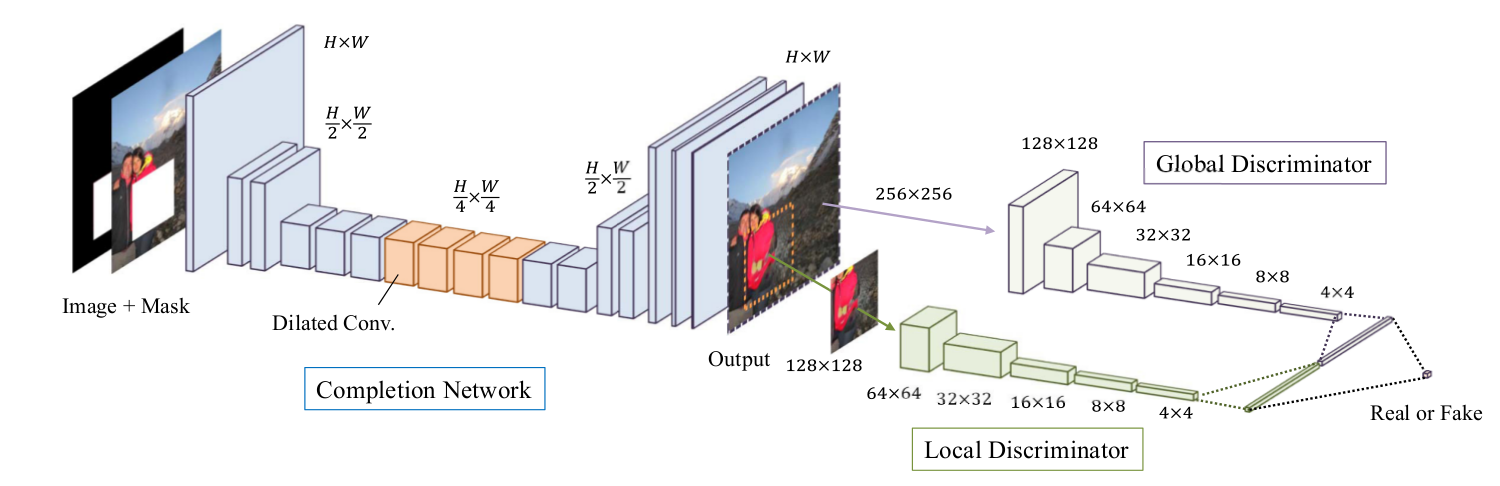
\includegraphics[width=1.0\textwidth]{network_overview.png}
    \caption{Overview of the architecture}
\end{figure}

\subsection{Entrainement}

\section{Observation sur des exemples}

\subsection{Dataset utilisé pour entrainement : Places2}
ça marche bien

\subsection{Visage (CelebA)}

\subsection{Problèmes}
\begin{itemize}
    \item visages
    \item trop près du bord
    \item mask rectangulaire vs difforme
\end{itemize}

Marche pas bien du tout car le model n'est pas entrainer dessus.
Ce model n'est pas disponible pour faire des test : TODO github photo

\section{Qu'est-ce qu'on peut changer pour observer les couches?}

\subsection{Batchnormlisation}


\subsection{Rajouter du bruit dans les couches}

\subsubsection{Test avec une image de référence}
Test et observation de la dégradation de l'inpainting

\section{Questions additionnelles}

Est-ce que la complétion vient d'un patch ou bien est-ce qu'elle est créée ? \\
Zero padding ? Vérifier sur les exemples.\\


\bibliographystyle{plain}
\bibliography{bib}

\end{document}
